% pygeek2026-ko.tex
% PyGeek 2026 submission — Korean short paper.
% Content transcribed verbatim from docs/research/paper-ko.md; this file
% is the typesetting layer only (see repo CLAUDE.md / task instructions).
% 구성은 지도교수 피드백(2026-08-08)에 따른 4절 체계:
%   1. 서론 / 2. 제안 방법(2.1~2.3) / 3. 성능평가(3.1~3.2) / 4. 결론
% 3쪽 압축판: 요인 분해 그림 삭제 → 표 1(실험 조건 구성)로 대체, 결과 표 12행→8행 축약,
%   구조도 그림 한 줄 노드 재제작(높이 -40%), 표 2와 중복되는 본문 통계 서술 제거.

\documentclass[10pt,a4paper,twocolumn]{article}

% ---------- fonts ----------
\usepackage{xetexko}
\latinparens            % ASCII 괄호·대괄호를 한글 글꼴이 아닌 본문(Times) 글꼴로 — 템플릿 표기와 일치
\setmainfont{Times New Roman}
\setmainhangulfont{Nanum Myeongjo}   % 템플릿의 바탕체(BatangChe) 미설치 → 동일 계열 명조체, 진짜 Bold 보유

% ---------- page geometry ----------
\usepackage[a4paper,left=1.78cm,right=1.78cm,top=1.78cm,bottom=1.78cm,%
            headheight=22pt,headsep=8pt,footskip=16pt,columnsep=1.27cm]{geometry}  % 수치는 PyGeek 공식 DOCX 템플릿의 pgMar/cols에서 추출

% ---------- misc packages ----------
\usepackage{fancyhdr}
\usepackage{graphicx}
\usepackage{amsmath}
\usepackage{unicode-math}
\setmathfont{STIX Two Math}   % Times 호환 수식 글꼴 (템플릿 본문 Times와 정합)
\usepackage{booktabs}
\usepackage{array}
\usepackage{url}
\urlstyle{same}   % URL·DOI도 본문 글꼴(Times)로 — 템플릿 참고문헌 표기와 일치
\Urlmuskip=0mu plus 1mu\relax          % 참고문헌 URL이 줄 어디서든 자연스럽게 끊기도록
\def\UrlBreaks{\do\/\do\-\do\.\do\:\do\_\do\?\do\=\do\&\do\a\do\b\do\c\do\d\do\e\do\f\do\g\do\h\do\i\do\j\do\k\do\l\do\m\do\n\do\o\do\p\do\q\do\r\do\s\do\t\do\u\do\v\do\w\do\x\do\y\do\z\do\0\do\1\do\2\do\3\do\4\do\5\do\6\do\7\do\8\do\9}   % URL·DOI도 본문 글꼴(Times)로 — 템플릿 참고문헌 표기와 일치
\usepackage{setspace}
\usepackage{textcomp}

\clubpenalty=10000\widowpenalty=10000   % 제목 직후 한 줄 고아·과부 줄 방지
\tolerance=1000
\emergencystretch=3em

% 두 폭 그림(figure*)이 페이지 상단에 자리 잡도록 허용
\renewcommand{\dbltopfraction}{0.95}
\renewcommand{\dblfloatpagefraction}{0.7}
\renewcommand{\topfraction}{0.95}
\renewcommand{\textfraction}{0.05}
\setcounter{dbltopnumber}{2}

% ---------- body typography: 10pt / 1.15 spacing / justified (default) ----------
\setstretch{1.15}
\setlength{\parindent}{0pt}
\setlength{\parskip}{1.2pt}

% ---------- running header / footer ----------
\pagestyle{fancy}
\fancyhf{}
\renewcommand{\headrulewidth}{0.6pt}
\renewcommand{\footrulewidth}{0pt}
\fancyhead[R]{\fontsize{10}{12}\selectfont 2026 International Conference on PyGeek (PyGeek 2026)}
\fancyfoot[R]{\thepage}

\fancypagestyle{firstpage}{%
  \fancyhf{}
  \fancyhead[L]{\fontsize{10}{12}\selectfont\parbox[b]{8cm}{2026 International Conference on PyGeek (PyGeek 2026)\\[1pt] Vol. xx, 2026}}
  \fancyhead[R]{\fontsize{10}{12}\selectfont ISSN (Online): 0000-0000}
  \renewcommand{\headrulewidth}{0.6pt}
  \fancyfoot[R]{\thepage}
}

% ---------- section heading macros (manual numbering, matches source text) ----------
\newcommand{\pgsec}[1]{\par\vspace{5pt}{\bfseries\fontsize{12}{14}\selectfont #1}\par\nobreak\vspace{2pt}\nobreak}
\newcommand{\pgsubsec}[1]{\par\vspace{4pt}{\bfseries\fontsize{12}{14}\selectfont #1}\par\nobreak\vspace{1pt}\nobreak}
\newcommand{\pgspecial}[1]{\par\vspace{5pt}\begin{center}{\bfseries\fontsize{12}{14}\selectfont #1}\end{center}\vspace{2pt}}

\begin{document}
\thispagestyle{firstpage}

% ======================================================================
% Full-width title block + abstract (single column, first page)
% ======================================================================
\twocolumn[
  \begin{center}
    \setstretch{1.0}
    {\fontsize{16}{20}\selectfont\bfseries 벡터 데이터베이스 마이그레이션에서 저장소 교체와 임베딩 배치의 효과를 분리하는 요인 분해 방법}\par
    \vspace{8pt}
    {\fontsize{16}{20}\selectfont\bfseries A Factor Decomposition Method for Separating Store Substitution and Embedding Placement Effects in Vector Database Migration}\par
  \end{center}
  \vspace{7pt}
  \noindent\rule{\linewidth}{0.6pt}\par
  \vspace{4pt}
  {\bfseries\fontsize{12}{14}\selectfont 초록}\par
  \vspace{3pt}
  \setstretch{1.15}
  {\fontsize{8}{9.6}\selectfont
  검색증강생성(RAG) 시스템의 벡터 계층을 다른 데이터베이스로 이전할 때, 그 효과는 통상 이전 전후 시스템의 종단 간 비교로 평가된다. 그러나 이 비교는 서로 독립적이지만 실무에서 함께 일어나는 두 변경, 즉 저장소 엔진의 교체와 임베딩 연산 위치의 이동을 한 측정값에 섞어 버려, 변화가 어느 요인 때문인지 가려낼 수 없게 만든다. 본 논문은 원본 시스템이 생성한 임베딩을 목표 저장소에 그대로 적재한 교량 조건(bridge condition)을 도입하여, 두 요인이 뒤섞인 하나의 비교를 한 번에 한 요인만 달라지는 두 개의 비교로 나누는 방법을 제안한다. 교량 조건은 재임베딩이 필요 없어 비용이 낮고 운영 서비스를 건드리지 않는다. 운영 중인 한국어 제품 리뷰 RAG 서비스(청크 1,347개, 질의 43건)에 적용한 결과, 저장소 교체에서는 검색 품질의 변화가 검출되지 않은 반면(상위 10개 Jaccard 0.971, 관련성 차이 $-$0.042, $p = 0.52$), 임베딩을 데이터베이스 내부로 이동한 변경은 유의하고 중간 크기의 효과를 보였다($p = 0.003$, Cohen's $d_z = 0.47$). 즉 관측된 변화는 사실상 전부 임베딩 배치 요인에서 비롯된다. 본 방법은 특정 제품의 우열을 평가하지 않으며 컨버지드 데이터베이스로의 이전 일반에 적용할 수 있다.
  \par}
  \vspace{5pt}
  {\bfseries\fontsize{10}{12}\selectfont 키워드: }{\fontsize{8}{9.6}\selectfont 검색증강생성, 벡터 데이터베이스, 인-데이터베이스 임베딩, 마이그레이션, 요인 분해}\par
  \vspace{6pt}
  \noindent\rule{\linewidth}{0.6pt}\par
  \vspace{7pt}
]

% ======================================================================
% 1. 서론
% ======================================================================
\pgsec{1. 서론}

검색증강생성(RAG) 시스템은 질의와 문서를 벡터로 변환하는 임베딩 모델, 벡터를 색인하고 검색하는 저장소, 검색 결과를 근거로 답변을 생성하는 언어모델로 구성된다 [1], [2]. 이 가운데 배포 이후 변경이 가장 잦은 구성 요소는 벡터 계층이다. 대표적인 변경 경로는 범용 관계형 데이터베이스에 벡터 확장을 결합한 구성에서, 벡터 타입과 추론 런타임을 안에 갖춘 컨버지드 데이터베이스, 즉 임베딩 계산까지 데이터베이스가 직접 처리하는 형태로 이전하는 것이다.

이러한 이전의 효과는 보통 이전 전과 후의 시스템 전체를 한 번에 견주는 종단 간 비교로 평가된다. 그러나 이 비교에서는 두 요인이 동시에 변경된다. 첫째는 벡터를 저장하고 검색하는 엔진과 색인 방식, 즉 저장소다. 둘째는 임베딩 연산을 외부 서비스가 수행하는지 데이터베이스 내부의 추론 런타임이 수행하는지를 가리키는 배치다. 거버넌스를 목적으로 이전할 때 임베딩까지 내부로 옮기는 구성이 선호되고, 모델을 내장하는 데이터베이스는 모델 파일 크기를 제한한다. 두 요인이 실무에서 함께 변경되는 이유다.

그 결과 종단 간 차이만 보아서는 변화가 어느 요인 때문인지 가려낼 수 없다. 품질이 떨어져도 저장소 탓인지 모델 탓인지 구분되지 않고, 변화가 없어도 두 요인이 서로 상쇄된 것인지 알 수 없다. 어느 경우든 인스턴스 등급이나 모델 크기 제약이 다른 환경에는 결론을 그대로 옮길 수 없다.

본 논문은 원본 시스템이 만들어 둔 임베딩을 목표 저장소에 그대로 적재한 중간 조건, 곧 교량 조건을 끼워 넣어, 두 요인이 뒤섞인 하나의 비교를 한 번에 한 요인만 달라지는 두 개의 비교로 나눈다. 제안 방법을 PostgreSQL 벡터 확장에서 내부 임베딩을 지원하는 컨버지드 데이터베이스로 이전한 한국어 리뷰 분석 서비스에 적용하고, 운영 코퍼스의 리뷰 조각(청크) 1,347개와 고정 질의 43건으로 측정하였다. 본 논문은 제품의 우열을 평가하지 않으며, 지연 수치는 제품이 아니라 측정 환경을 반영한다.

% ======================================================================
% 2. 제안 방법
% ======================================================================
\pgsec{2. 제안 방법}

% Figures 1 & 2 (system architectures, section 2.1)
\begin{figure*}[t]
\centering
\begin{minipage}[t]{0.45\textwidth}
  \centering
  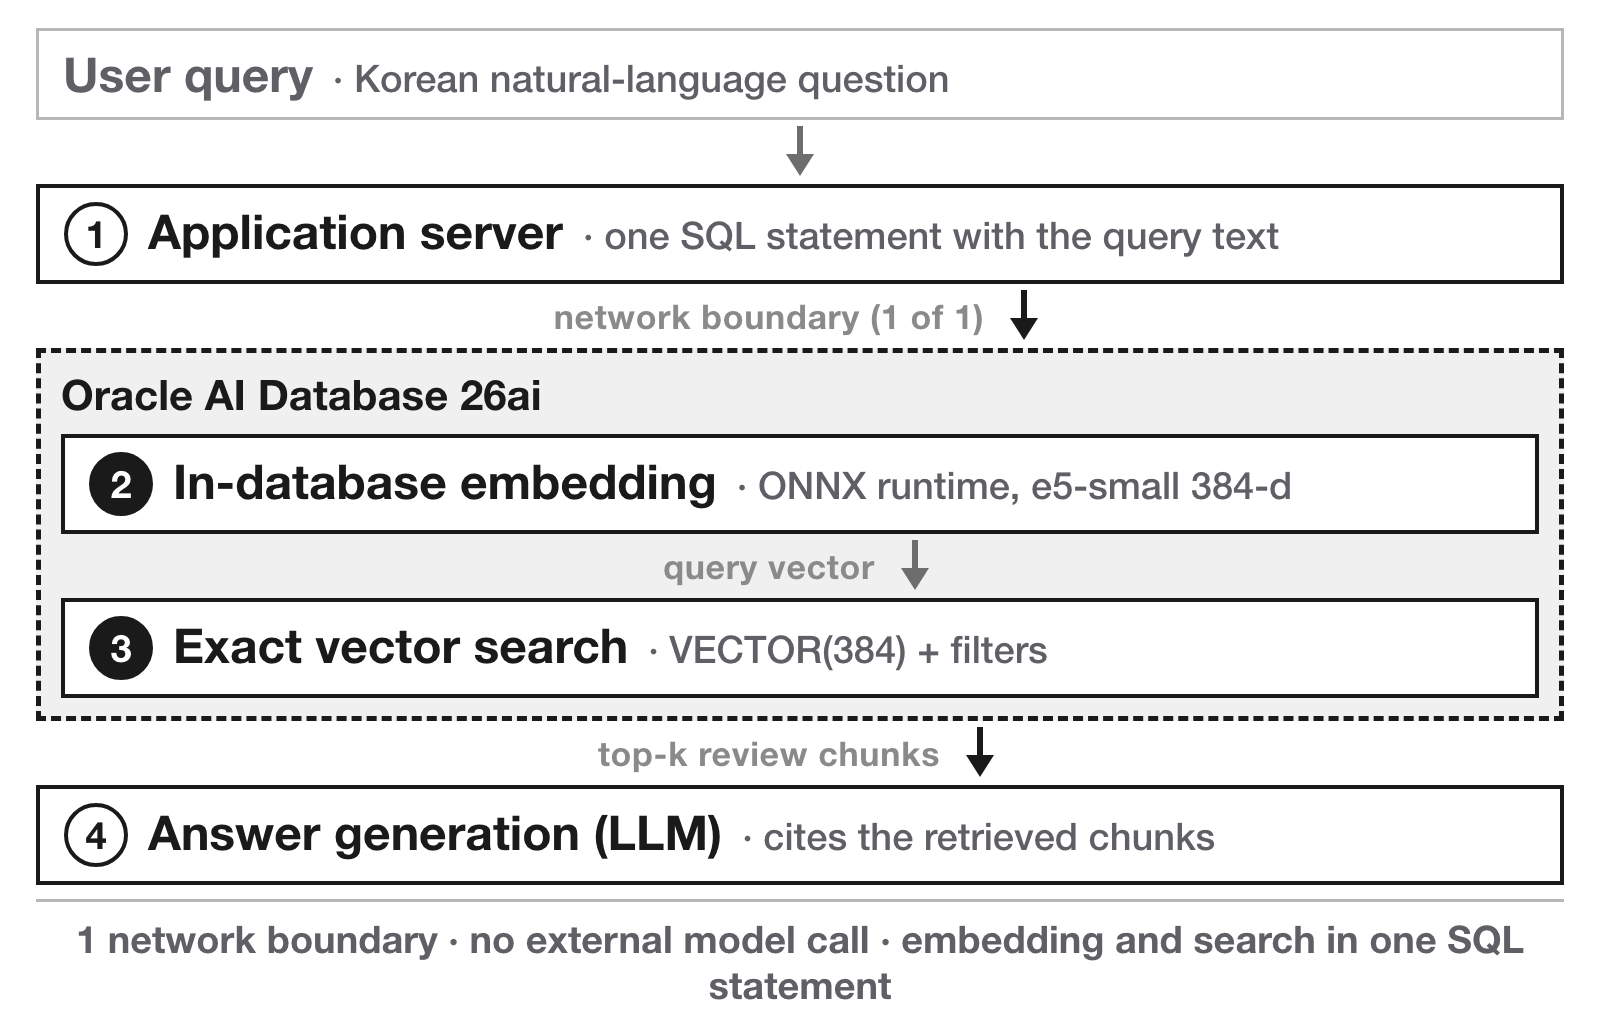
\includegraphics[width=\linewidth]{../../figures/paper-fig1-arch-oracle.png}\par
  \vspace{5pt}
  {\fontsize{8}{9.6}\selectfont 그림 1. Oracle 기반 시스템 구조\\
  Fig. 1. Oracle-based system architecture}
\end{minipage}\hfill
\begin{minipage}[t]{0.45\textwidth}
  \centering
  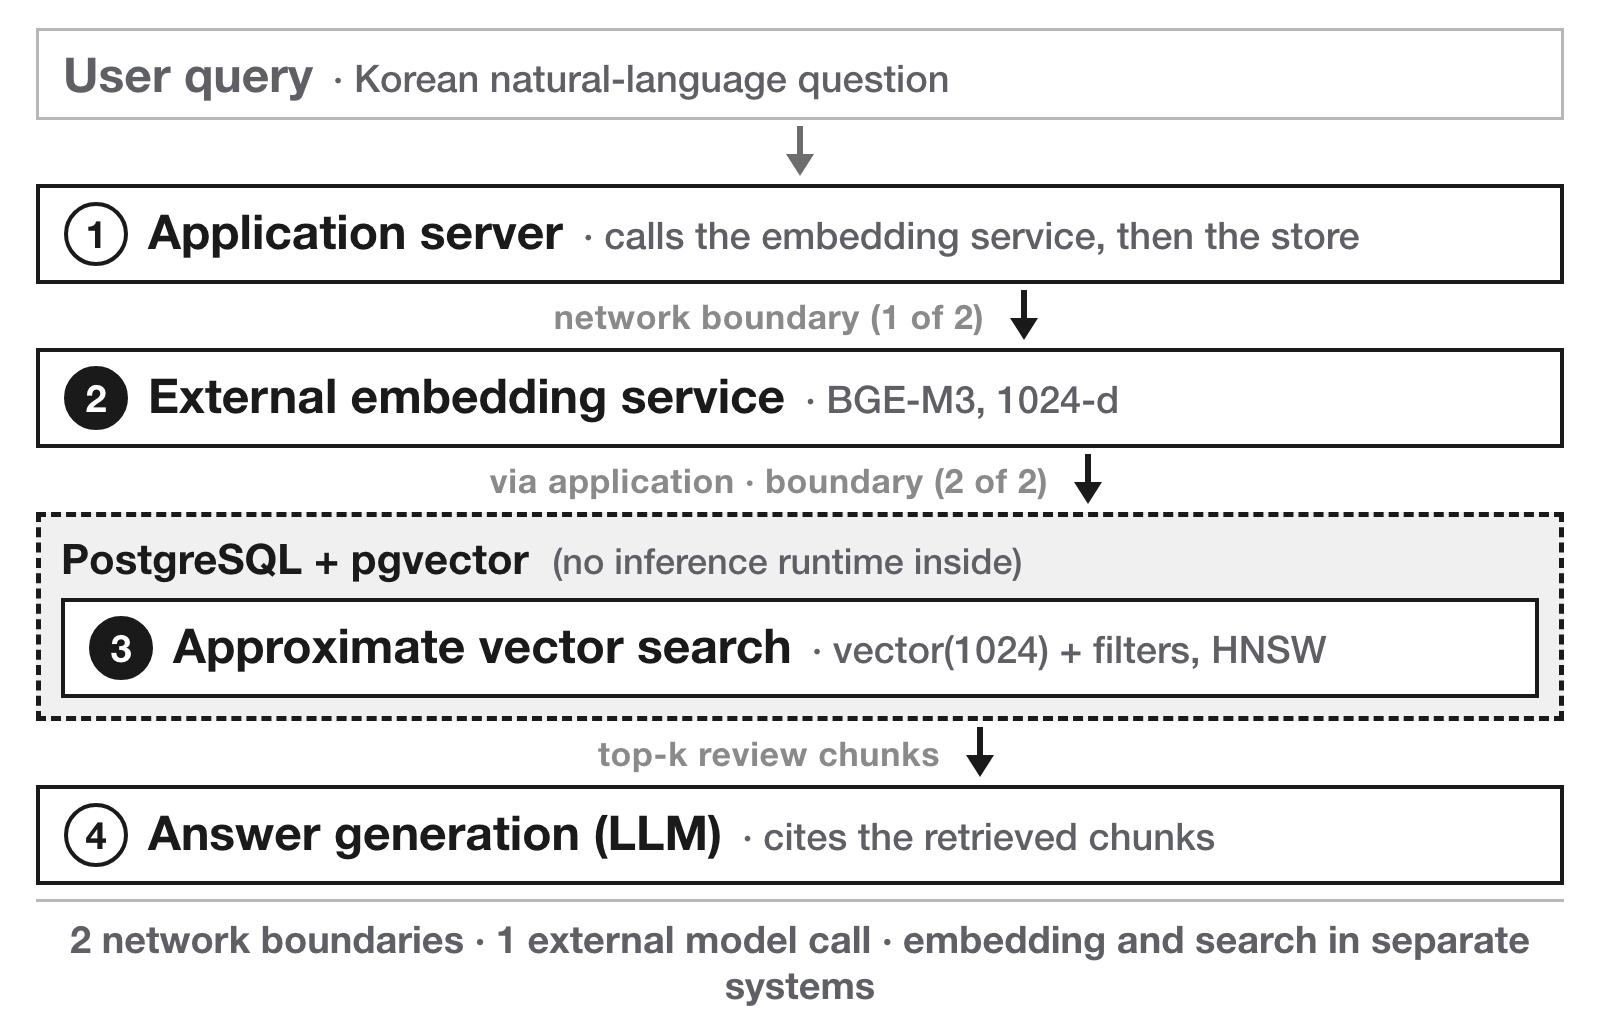
\includegraphics[width=\linewidth]{../../figures/paper-fig2-arch-pgvector.png}\par
  \vspace{5pt}
  {\fontsize{8}{9.6}\selectfont 그림 2. PostgreSQL 기반 시스템 구조\\
  Fig. 2. PostgreSQL-based system architecture}
\end{minipage}
\end{figure*}

\pgsubsec{2.1 시스템 구조도}

대상 시스템은 한국어 제품 리뷰를 검색하여 근거를 인용한 답변을 생성한다. 두 구조 모두 질의 입력, 질의 임베딩, 벡터 검색, 답변 생성의 네 단계로 동작한다. 검색은 벡터 유사도에 메타데이터 필터와 출처 기반 우선순위를 결합한 하이브리드 방식이며, 세 조건에서 이 규칙과 파라미터를 동일하게 유지하였다. 양쪽 모두 단일 SQL 문으로 표현되므로 애플리케이션 로직을 그대로 둔 채 저장소와 임베딩 배치만 교체할 수 있다.

그림 1은 Oracle 기반 구조다. 애플리케이션은 질의 문자열을 담은 SQL 문 하나를 전달하고(단계 1), 데이터베이스는 내장 ONNX 추론 런타임으로 질의를 384차원 벡터로 변환한 뒤(단계 2) 같은 SQL 문 안에서 VECTOR 컬럼에 대한 정확 검색과 메타데이터 필터링을 수행한다(단계 3). 반환된 상위 $k$개 청크를 언어모델이 인용해 답변을 생성한다(단계 4).

그림 2는 PostgreSQL 기반 구조다. 애플리케이션은 외부 임베딩 서비스를 호출해 질의를 1024차원 벡터로 변환하고(단계 2), 그 벡터를 인자로 검색을 요청한다(단계 3). 저장소는 HNSW 근사 색인으로 후보를 탐색한 뒤 같은 필터를 적용하며, 이후 단계는 그림 1과 같다.

두 구조는 저장소와 임베딩 배치라는 두 가지가 동시에 다르다. 하나는 벡터를 어느 엔진이 어떤 색인 방식으로 보관하는가이고, 다른 하나는 임베딩을 데이터베이스 밖에서 계산하는가 안에서 계산하는가다. 종단 간 비교만으로는 이 둘 중 어느 쪽이 차이를 만들었는지 알 수 없다. 이어지는 두 절에서 각 구조의 특징을 이 두 관점으로 정리하고, 3절에서 둘을 떼어 내는 방법을 제시한다.

\pgsubsec{2.2 Oracle 구조의 특징}

첫째, 네이티브 VECTOR 타입과 내장 ONNX 추론 런타임을 제공하므로 임베딩과 검색이 하나의 SQL 문으로 결합된다 [3]. 둘째, 후보를 미리 좁히는 근사 색인 없이 모든 벡터를 다 비교하는 정확 검색을 수행하므로, 색인 때문에 정답을 놓치는 일이 없다. 셋째, 네트워크 경계가 하나로 줄어 질의와 검색 결과가 데이터베이스 안에 머무르므로 암호화·감사 같은 통제가 검색 경로 전체에 적용된다. 넷째, 내장 모델은 데이터베이스가 허용하는 모델 파일 크기 상한을 따르며, 본 환경에서 그 상한 안의 최대 다국어 모델은 multilingual-e5-small(384차원)이었다 [4].

\pgsubsec{2.3 PostgreSQL 구조의 특징}

첫째, 벡터 검색을 확장 모듈(pgvector)로 제공하며 추론 런타임을 포함하지 않는다 [5]. 임베딩 모델을 저장소와 따로 고를 수 있어 크기 제약이 없고, 본 구조에서는 1024차원 BGE-M3를 쓴다 [6]. 둘째, 후보를 좁혀 가며 탐색하는 HNSW 근사 색인을 쓰므로 데이터가 늘어도 검색 시간이 완만하게 증가하는 대신, 정답을 일부 놓칠 수 있다 [7]. 셋째, 임베딩이 외부에서 수행되므로 질의 텍스트가 저장소 경계를 벗어나고 네트워크 왕복이 한 번 더 든다.

% ======================================================================
% 3. 성능평가
% ======================================================================
\pgsec{3. 성능평가}

\pgsubsec{3.1 실험 환경}

본 실험에서는 검색 구성을 세 요소의 조합 $(S, E, P)$로 표기한다. $S$는 저장소, $E$는 임베딩 모델, $P$는 임베딩의 실행 위치다. 2절의 두 구조를 그대로 비교하면 $(S_0, E_0, \text{외부})$와 $(S_1, E_1, \text{내부})$를 비교하게 되어 세 좌표가 모두 달라 요인별 기여를 분리할 수 없다. 그래서 여기에 $(S_1, E_0, \text{외부})$, 즉 목표 저장소를 쓰되 벡터는 원본 시스템이 생성한 것을 그대로 적재한 교량 조건을 추가하였으며, 세 조건의 구성은 표 1과 같다. 교량 조건은 벡터를 다시 계산할 필요가 없다. 운영 중인 컬럼은 그대로 둔 채 벡터 컬럼 하나를 더 만들어 채우면 되므로, 준비 비용은 한 번의 일괄 적재뿐이고 운영 서비스도 건드리지 않는다.

% Table 1 (experimental conditions, section 3.1)
\begin{table}[t]
\centering
{\fontsize{8}{9.6}\selectfont 표 1. 실험 조건 구성\\
Table 1. Experimental conditions}
\vspace{4pt}

\fontsize{6.9}{8.1}\selectfont
\setlength{\tabcolsep}{2pt}
\renewcommand{\arraystretch}{0.95}
\begin{tabular}{@{}l>{\raggedright\arraybackslash}p{1.85cm}>{\raggedright\arraybackslash}p{1.85cm}>{\raggedright\arraybackslash}p{1.85cm}@{}}
\toprule
 & A (기준선) & B (교량 조건) & C (이전 완료) \\
\midrule
저장소 & PostgreSQL + pgvector & Oracle 26ai & Oracle 26ai \\
임베딩 모델 & BGE-M3 (1024) & BGE-M3 (1024) & e5-small (384) \\
임베딩 배치 & 외부 & 외부 & 내부 \\
벡터 검색 & HNSW 근사 & 정확 & 정확 \\
\bottomrule
\end{tabular}

\vspace{4pt}
{\fontsize{6.9}{8.1}\selectfont A$\rightarrow$B는 저장소 요인만, B$\rightarrow$C는 배치 요인만 변화시킨다. e5-small은 multilingual-e5-small이다.}
\end{table}

다만 조건 C에서는 배치를 옮기면 모델도 같이 바뀐다. 2.2절의 파일 크기 상한 때문에 원본 모델을 데이터베이스 안에 넣을 수 없기 때문이다. 내부 배치를 고르면 이 상한도 함께 받아들여야 하므로 이 묶임은 일부러 두었다. 둘을 떼어 보려면 작은 모델을 데이터베이스 밖에서 돌리는 $(S_1, E_1, \text{외부})$ 조건이 하나 더 필요하며, 이는 후속 과제로 남긴다.

코퍼스는 운영 서비스의 단일 제품 도메인 리뷰 청크 1,347개이며, 두 저장소에 똑같이 적재한 뒤 청크 식별자가 1대1로 맞물리는지 미리 확인하였다. 질의는 한국어 43건으로 고정했으며, 운영 로그에서 뽑은 13건과 서비스가 다루는 평가 관점·구매 여정 단계를 고루 포괄하도록 만든 합성 질의 30건이다.

측정 지표는 세 가지다. 첫째는 검색 결과의 일치도다. 같은 질의에 대해 두 조건이 내놓은 상위 10개가 얼마나 겹치는지(Jaccard), 그 순위가 얼마나 비슷한지(Spearman 순위상관), 그리고 교량 조건의 정확 검색을 정답으로 삼았을 때 기준선이 그중 몇 개를 되찾는지(Recall@10)를 본다. 둘째는 검색된 근거의 관련성이다. 대형 언어모델이 상위 5개 청크를 0--2점으로 채점하며 [8], 조건당 215건을 채점해 질의별 평균을 낸 뒤 같은 질의끼리 짝지어 비교한다. 셋째는 질의 하나를 처리하는 데 걸린 실제 시간이다.

목표 데이터베이스는 가장 낮은 등급의 무료 인스턴스(Always Free, RAM 2GB)에서, 외부 임베딩 서비스는 로컬 노트북(Apple M5 Pro)에서 동작하였다. 신뢰구간은 측정값을 10,000번 다시 뽑는 부트스트랩 방식으로 구하였다.

\pgsubsec{3.2 실험 결과}

요인별 측정 결과를 표 2에 정리하였다.

% Table 2 (results, section 3.2)
\begin{table}[t]
\centering
{\fontsize{8}{9.6}\selectfont 표 2. 요인별 측정 결과\\
Table 2. Results by factor}
\vspace{4pt}

\fontsize{6.9}{8.1}\selectfont
\setlength{\tabcolsep}{3pt}
\begin{tabular}{@{}lcc@{}}
\toprule
측정 항목 & A $\rightarrow$ B (저장소) & B $\rightarrow$ C (배치) \\
\midrule
상위 10개 Jaccard [95\% CI] & 0.971 [0.946, 0.992] & 0.175 [0.133, 0.221] \\
Spearman 순위상관 & 0.958 & --- \\
Recall@10 (정확 검색 대비) & 0.984 & --- \\
관련성 점수 (0--2) & 1.228 $\rightarrow$ 1.270 & 1.270 $\rightarrow$ 1.014 \\
대응 차이 [95\% CI] & $-$0.042 [$-$0.172, 0.084] & 0.256 [0.098, 0.423] \\
유의성 / 효과 크기 $d_z$ & $p = 0.523$ / $-$0.098 & $p = 0.003$ / 0.473 \\
평균 검색 지연 (ms) & 150.2 $\rightarrow$ 110.0 & 110.0 $\rightarrow$ 947.0 \\
외부 호출 / 네트워크 경계 & 1$\rightarrow$1 / 2$\rightarrow$2 & 1$\rightarrow$0 / 2$\rightarrow$1 \\
\bottomrule
\end{tabular}

\vspace{4pt}
{\fontsize{6.9}{8.1}\selectfont 관련성은 43개 질의의 질의별 평균(조건당 채점 215건)이며 $p$값은 대응표본 $t$검정이다.}
\end{table}

먼저 순위 일치도를 보면, 동일한 벡터를 적재한 두 저장소는 43개 질의 중 37개에서 상위 10개가 완전히 일치했고 최솟값도 0.667이었다. 기준선이 근사 색인 탓에 놓친 결과는 약 1.6\%다.

저장소 요인에서는 관련성 점수를 같은 질의끼리 짝지어 비교한 차이가 통계적으로 유의하지 않았고 효과 크기도 무시할 수준이었다($t(42) = -0.643$). 점수가 같은 질의를 제외한 28개 질의의 Wilcoxon 검정도 같은 결론이다($p = 0.908$).

한편 ``차이가 없다''가 곧 우리의 주장이므로, $p$값이 유의하지 않다는 사실에만 기대지 않고 동등성 자체를 따로 검정하였다 [9]. 차이가 $\pm$0.15점 안에 드는지 보는 두 단측검정 결과는 $p = 0.052$로, 신뢰구간 하한 $-$0.172가 이 범위를 벗어나 유의수준을 충족하지 못하였다. 따라서 동등성이 입증된 것이 아니라 효과가 검출되지 않았고 그 크기가 작은 범위로 제한된다고 보고한다. 다만 구간이 벗어난 방향이 목표 저장소의 관련성이 더 높은 쪽이므로 저장소 교체로 품질이 저하되었다고 볼 근거는 없다.

반면 저장소와 검색 방식이 동일한 B와 C 사이에서는 결과가 크게 달라진다. 상위 10개 Jaccard가 0.175로 낮아져 동일한 질의에 대해 대부분 다른 근거를 검색하며, 관련성 점수는 1.270에서 1.014로 감소한다. 이 차이는 유의하고 효과 크기는 중간 수준이며($t(42) = 3.104$), 점수가 같은 질의를 제외한 38개 질의의 Wilcoxon 검정도 같은 결론이다($p = 0.006$). A에서 B로의 변화에서 저장소 효과가 검출되지 않았으므로 종단 간 품질 변화는 사실상 전부 배치 요인과 거기 딸려 온 모델 용량 제약 때문이다. 종단 간 비교만 했다면 약 20\%의 관련성 감소를 저장소 탓으로 돌렸을 것이고, 그 진단에서 나오는 저장소 원복은 품질을 되돌리지 못한다.

검색 지연에서는 C와 B의 비율이 중앙값 기준 8.27배로 나타났다(Wilcoxon $p < 0.001$). C의 증가는 내부 임베딩 방식 자체의 특성이 아니라 무료 등급 인스턴스에서 추론이 수행된 결과이므로 상위 등급 하드웨어로 일반화할 수 없다. 한편 A와 B는 같은 외부 서비스로 같은 벡터를 만들므로 질의 임베딩 시간을 1회만 재어 두 조건에 공통 적용하였고, 따라서 둘의 지연 차이는 저장소 검색 시간만 반영한다.

끝으로 질의 43건 중 30건이 합성이므로 실제 질의 13건과 다르게 행동하지 않는지 확인하였다. 관련성 점수는 합성 부분집합에서 체계적으로 낮았으므로(A: 1.147 대 1.415, $p = 0.045$; C: 0.880 대 1.323, $p = 0.007$; Mann--Whitney) 관련성의 절대 수준을 서비스 품질로 읽어서는 안 된다. 반면 원인을 가리는 근거인 순위 일치도에는 두 부분집합 간 유의한 차이가 없었다($p = 0.441$, $p = 0.570$). 절대 점수는 질의 출처를 타지만 원인을 가리는 결론은 양쪽에서 같다.

% ======================================================================
% 4. 결론
% ======================================================================
\pgsec{4. 결론}

교량 조건 하나만 추가하면 종단 간 비교를 두 개의 단일 요인 비교로 분리할 수 있다. 운영 중인 한국어 리뷰 RAG 서비스에 적용한 결과 저장소 요인의 효과는 검출되지 않았고, 관측된 변화 전체가 배치 요인에서 비롯되었다. 배치 변경은 성능이 아니라 거버넌스의 교환이다. 질의와 리뷰 텍스트가 데이터베이스 경계 안에 머무르는 대신 모델의 용량 제약과 데이터베이스 등급의 추론 성능을 받아들여야 한다. 따라서 저장 데이터의 거버넌스만이 목적이라면 저장소만 교체하면 되고, 질의 경로까지 경계 안에 두어야 한다면 내장 가능한 최대 모델이 그 도메인에 충분한지를 먼저 확인해야 한다. 교량 조건은 이전을 실행하기 전에 그 확인을 가능하게 한다.

한계는 다음과 같다. 단일 한국어 코퍼스 1,347개 청크를 대상으로 하였고, 관련성 채점에 사람 평가자를 포함하지 않았으며, 입문 등급 인스턴스에서 측정하였다. 또한 3.1절에서 밝혔듯 배치와 모델 용량이 구성상 묶여 있으며, 저장소 요인의 결과는 동등함을 입증한 것이 아니다.

% ======================================================================
% References
% ======================================================================
\pgspecial{참고문헌}

{\setstretch{1.0}\setlength{\parskip}{0pt}\fontsize{8}{9.2}\selectfont\raggedright

\noindent\hangindent=0.5cm\hangafter=1
[1] P. Lewis et al., ``Retrieval-augmented generation for knowledge-intensive NLP tasks,'' Advances in Neural Information Processing Systems, vol. 33, pp. 9459-9474, 2020.
\par\vspace{0pt}

\noindent\hangindent=0.5cm\hangafter=1
[2] Y. Gao et al., ``Retrieval-augmented generation for large language models: A survey,'' arXiv preprint arXiv:2312.10997, 2023.
\par\vspace{0pt}

\noindent\hangindent=0.5cm\hangafter=1
[3] Oracle, ``Oracle AI Vector Search User's Guide,'' Oracle AI Database 26ai documentation, Available: \url{https://docs.oracle.com/en/database/oracle/oracle-database/26/vecse/}, 2026, [Accessed: Aug. 8, 2026].
\par\vspace{0pt}

\noindent\hangindent=0.5cm\hangafter=1
[4] L. Wang, N. Yang, X. Huang, L. Yang, R. Majumder, and F. Wei, ``Multilingual E5 text embeddings: A technical report,'' arXiv preprint arXiv:2402.05672, 2024.
\par\vspace{0pt}

\noindent\hangindent=0.5cm\hangafter=1
[5] pgvector, ``pgvector: Open-source vector similarity search for Postgres,'' GitHub repository, Available: \url{https://github.com/pgvector/pgvector}, 2026, [Accessed: Aug. 8, 2026].
\par\vspace{0pt}

\noindent\hangindent=0.5cm\hangafter=1
[6] J. Chen, S. Xiao, P. Zhang, K. Luo, D. Lian, and Z. Liu, ``M3-Embedding: Multi-linguality, multi-functionality, multi-granularity text embeddings through self-knowledge distillation,'' Findings of the Association for Computational Linguistics: ACL 2024, Bangkok, Thailand, pp. 2318-2335, \url{https://doi.org/10.18653/v1/2024.findings-acl.137}, Aug., 2024.
\par\vspace{0pt}

\noindent\hangindent=0.5cm\hangafter=1
[7] Y. A. Malkov and D. A. Yashunin, ``Efficient and robust approximate nearest neighbor search using hierarchical navigable small world graphs,'' IEEE Transactions on Pattern Analysis and Machine Intelligence, vol. 42, no. 4, pp. 824-836, \url{https://doi.org/10.1109/TPAMI.2018.2889473}, 2020.
\par\vspace{0pt}

\noindent\hangindent=0.5cm\hangafter=1
[8] L. Zheng et al., ``Judging LLM-as-a-Judge with MT-Bench and Chatbot Arena,'' Advances in Neural Information Processing Systems 36 (NeurIPS 2023), Datasets and Benchmarks Track, 2023.
\par\vspace{0pt}

\noindent\hangindent=0.5cm\hangafter=1
[9] D. Lakens, ``Equivalence tests: A practical primer for t tests, correlations, and meta-analyses,'' Social Psychological and Personality Science, vol. 8, no. 4, pp. 355-362, \url{https://doi.org/10.1177/1948550617697177}, 2017.
\par
}

\end{document}
